\Exhibit{Lehasoft}{%
    Download statistics for \mrls hobby computer games in 2002--2003\WithTr%
}

In the early and mid-2000s,
one of the popular software websites in Russia was download.ru.

It has been reorganized since, and the old data was destroyed.
These screenshots on Archive.org show archived versions (2002--2003)
of download statistics of \mrls computer games
(see the proof of authorship just after these statistics screenshots):

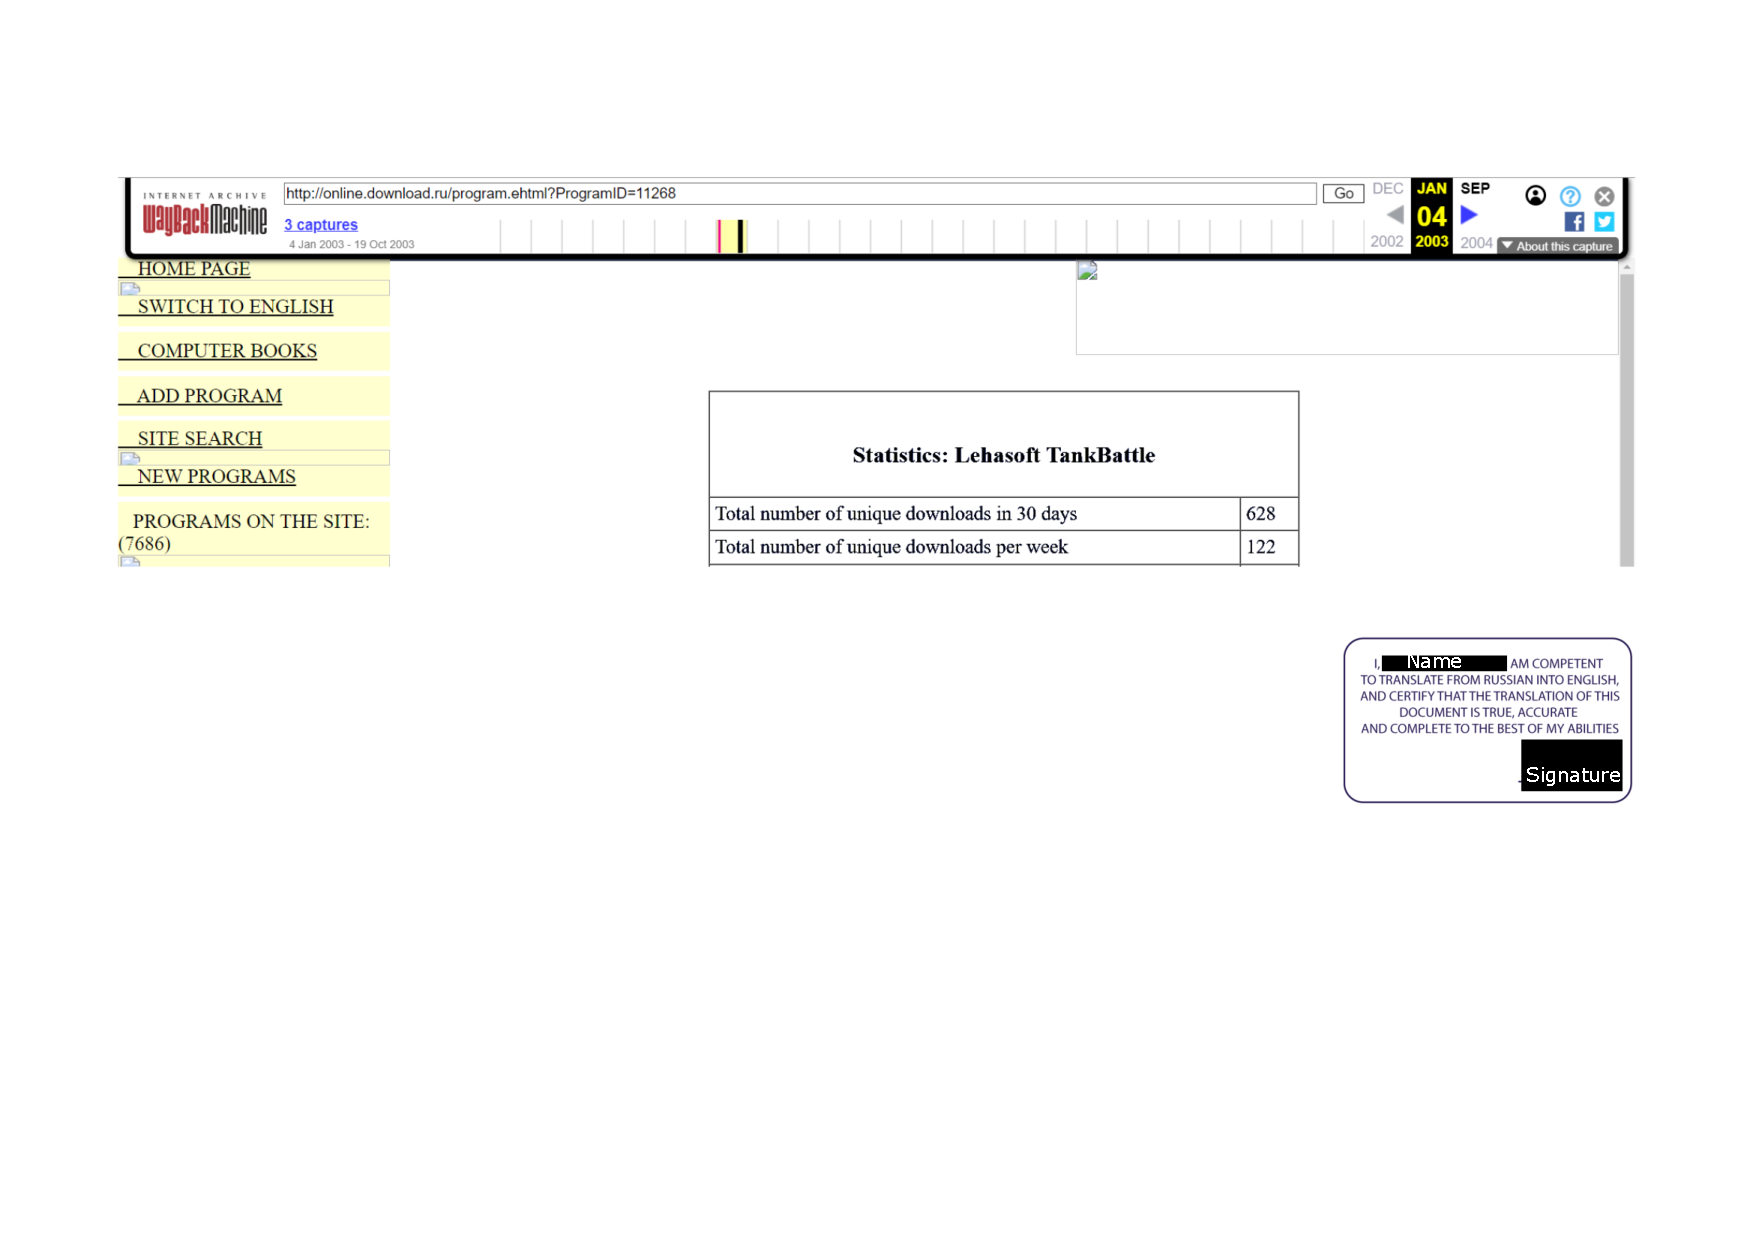
\includepdf[pages=-,angle=90]{tankbattle-downloads_eng_ai_public}
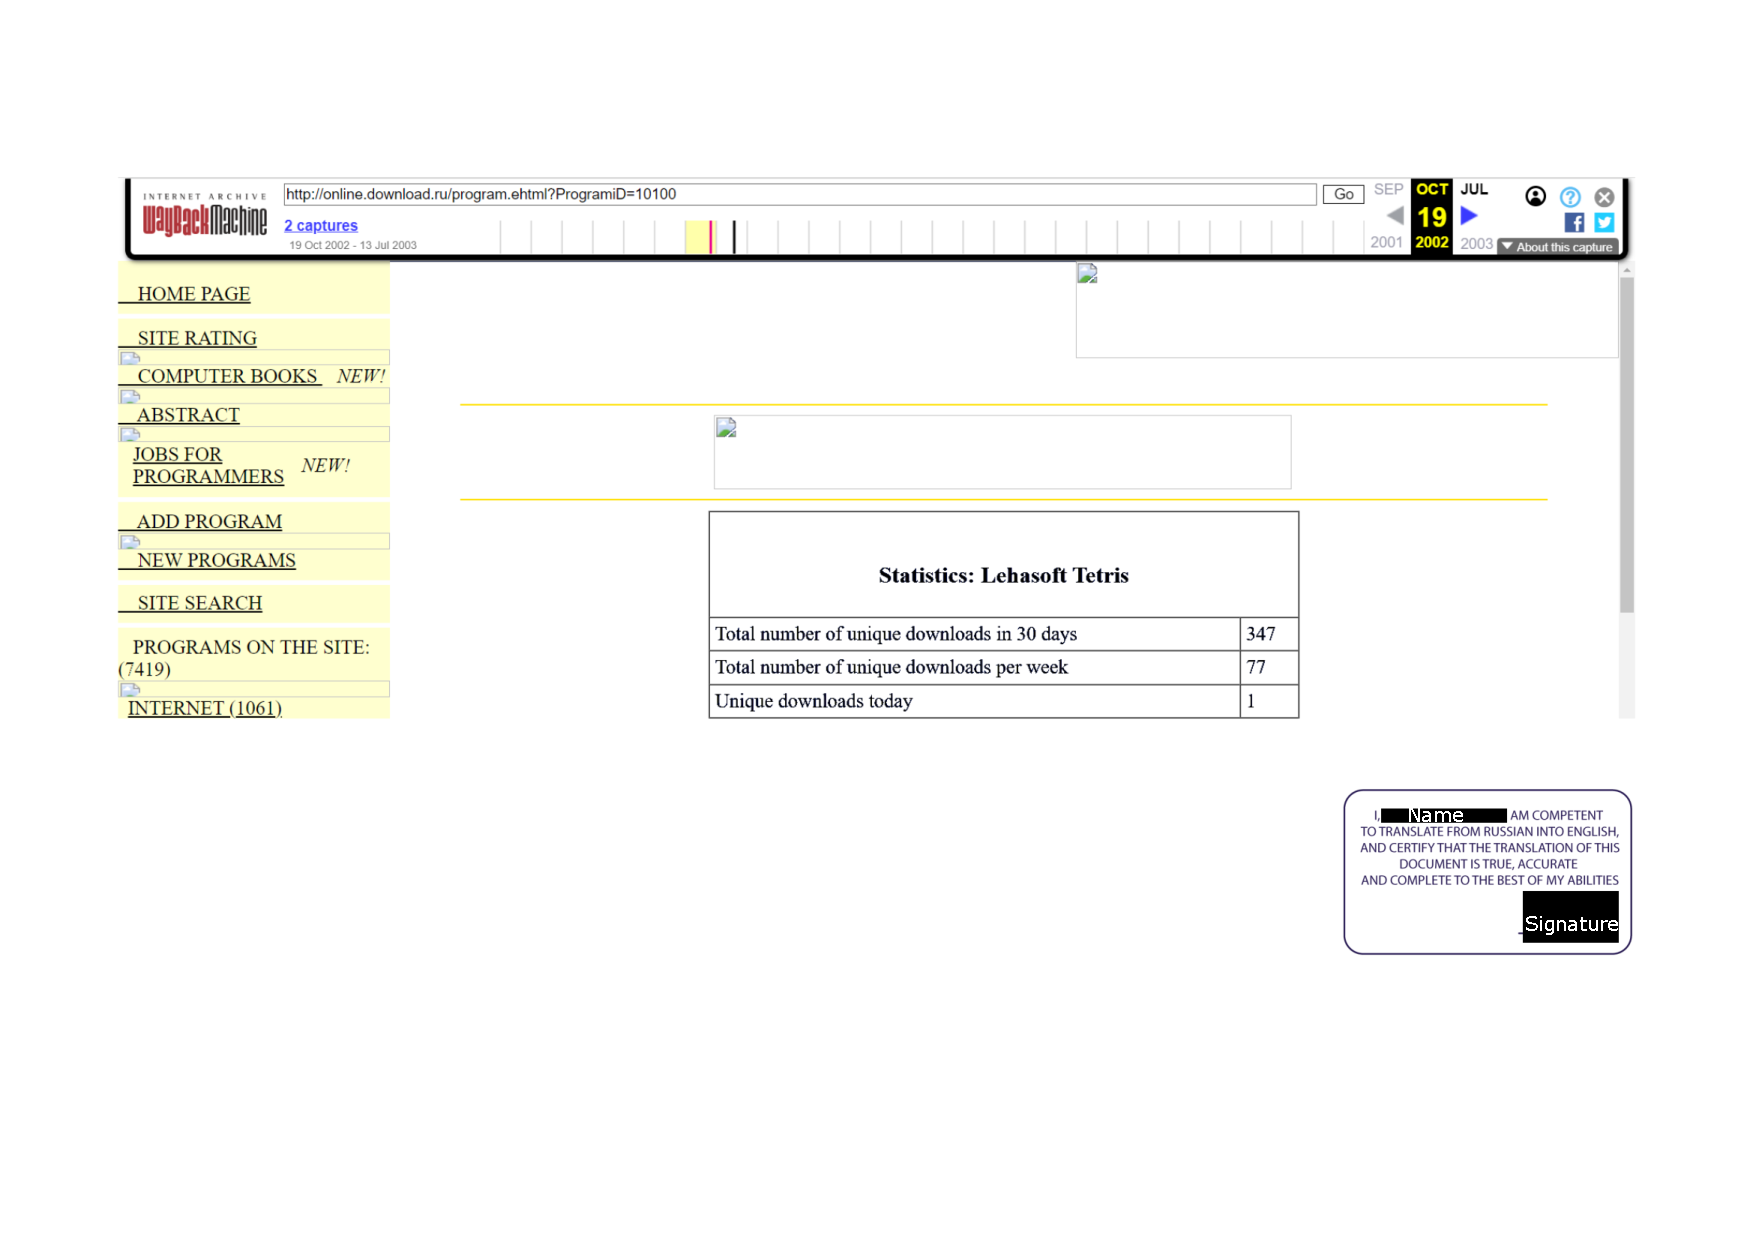
\includepdf[pages=-,angle=90]{tetris-downloads_eng_ai_public}
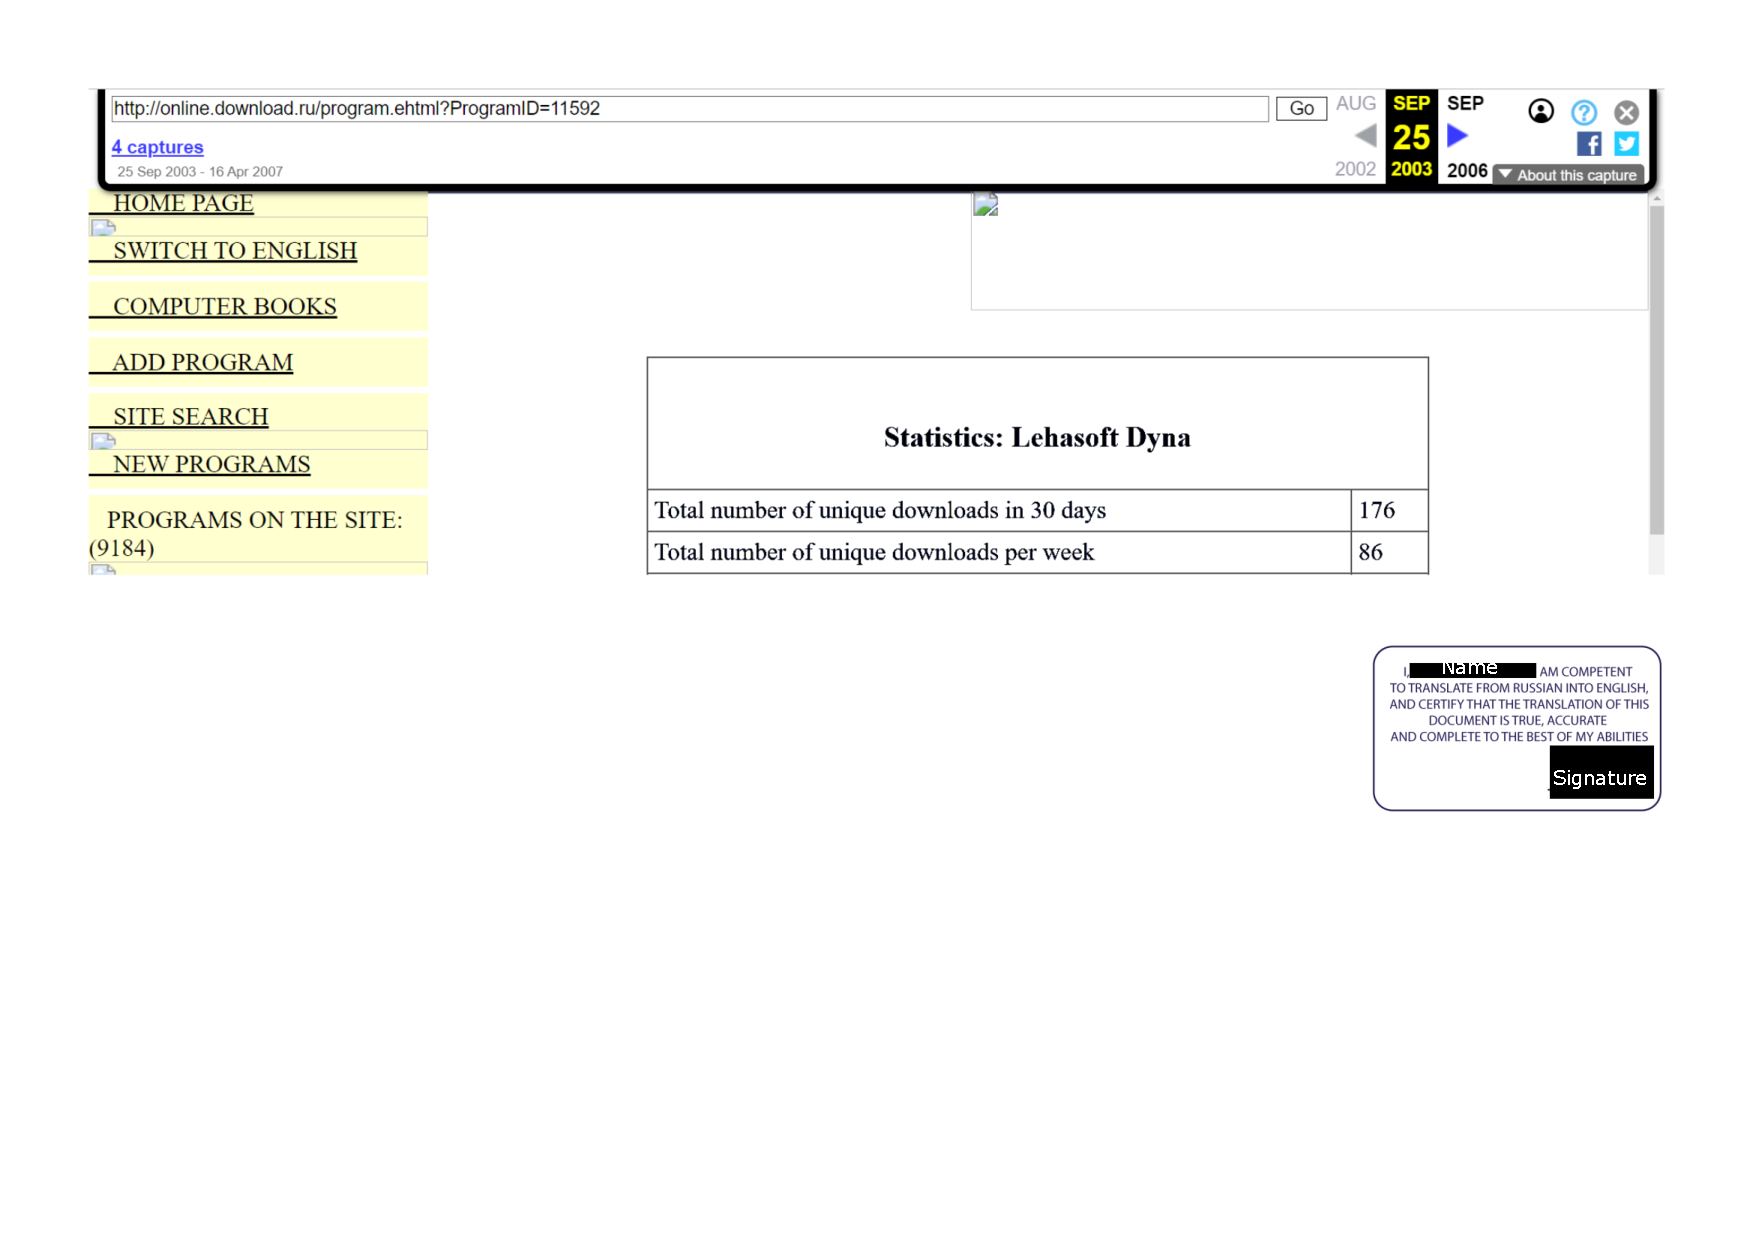
\includepdf[pages=-,angle=90]{dyna-downloads_eng_ai_public}

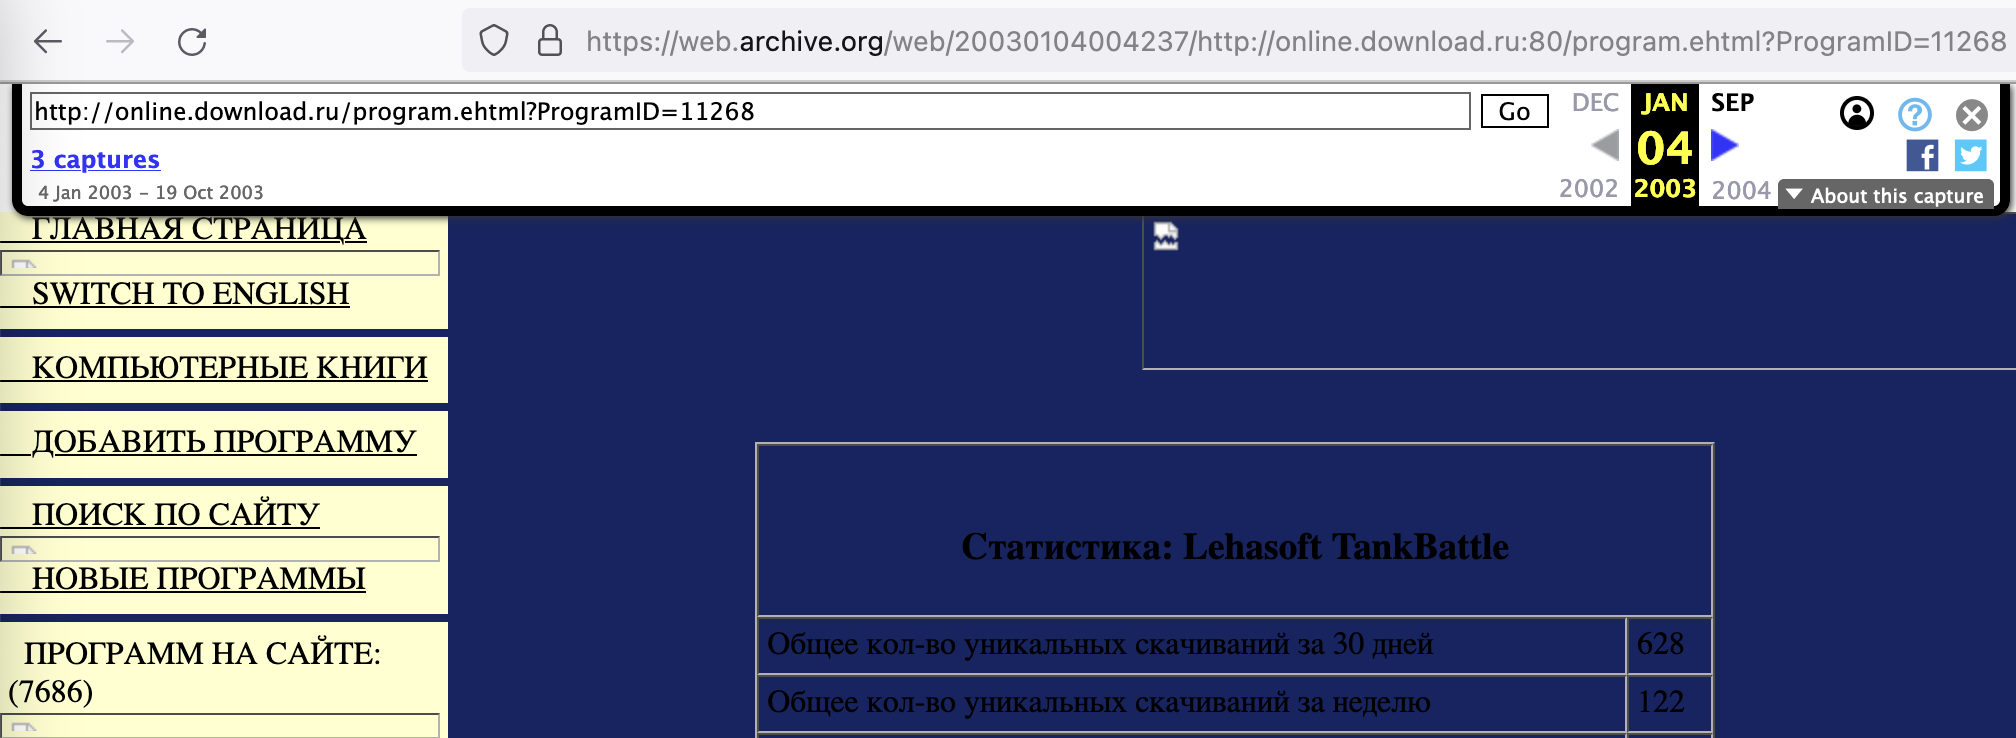
\includegraphics[width=40em]{tankbattle-downloads}

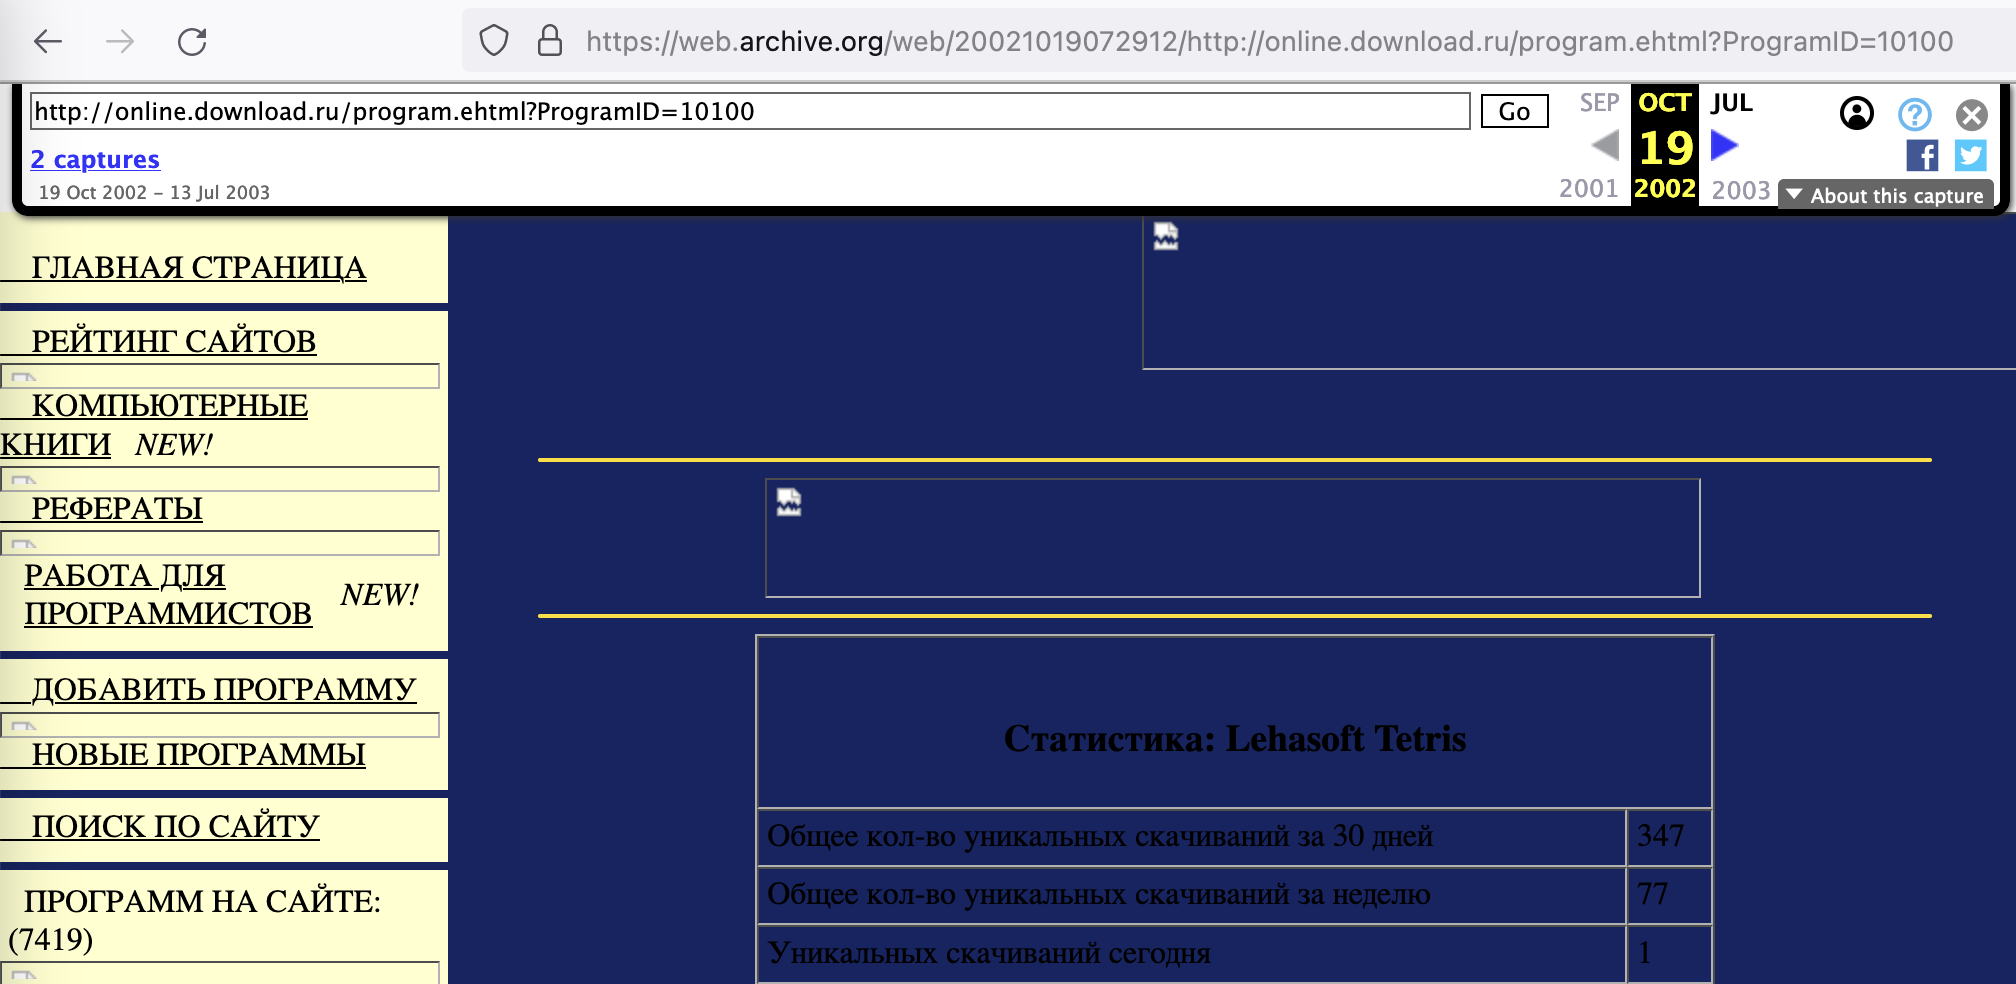
\includegraphics[width=40em]{tetris-downloads}

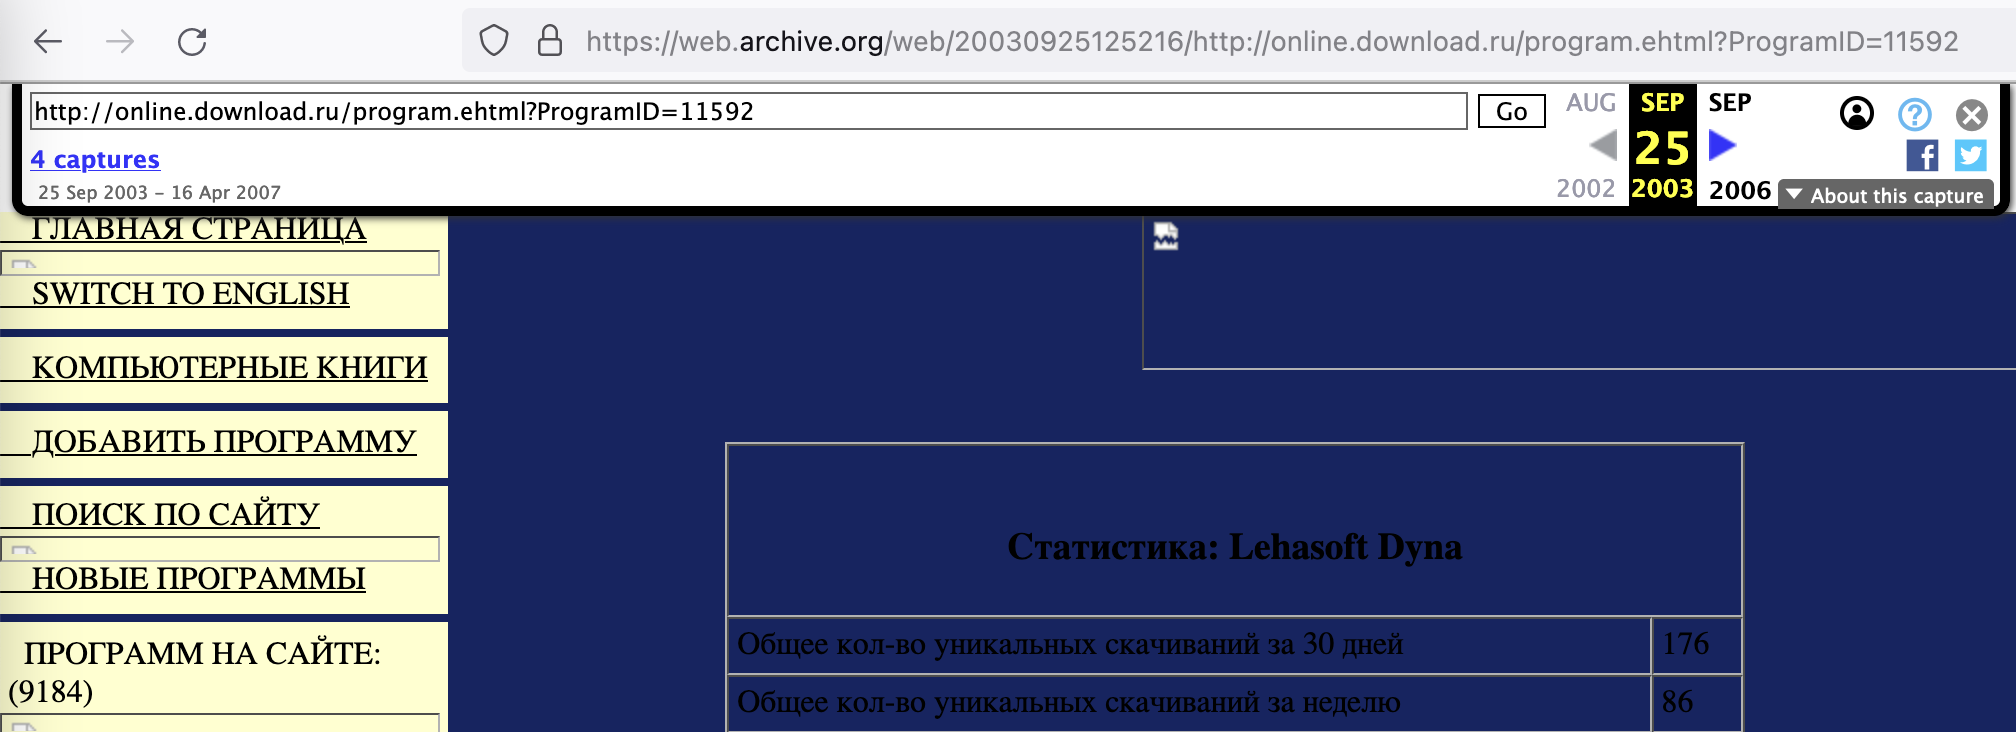
\includegraphics[width=40em]{dyna-downloads}

These games were published under an alias of `Lehasoft'
(`Leha' is the informal for `Alexey' in Russian),
which \mrl was using back then.
His authorship is proven by the archived version of his own website from 2002:

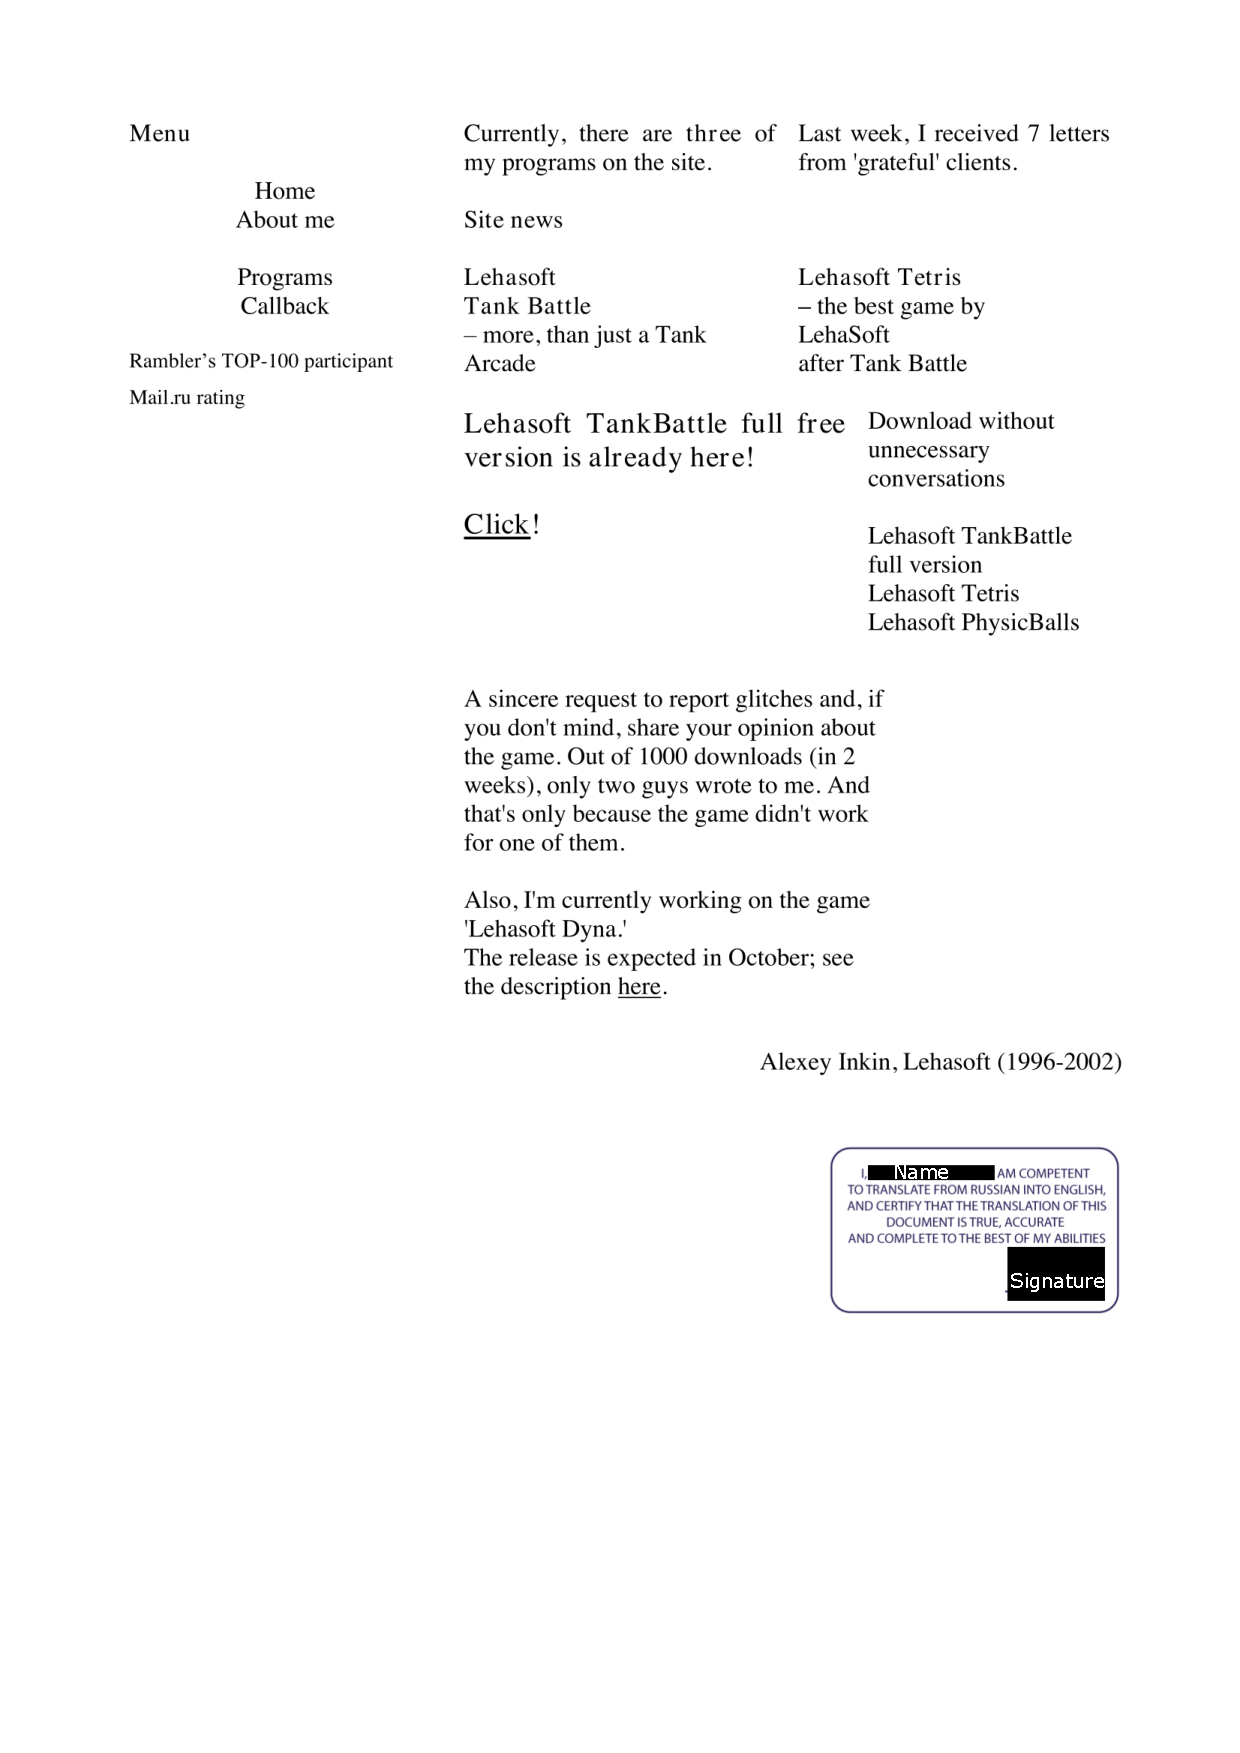
\includepdf[pages=-]{lehasoft-hotbox_eng_public}

\begin{center}
    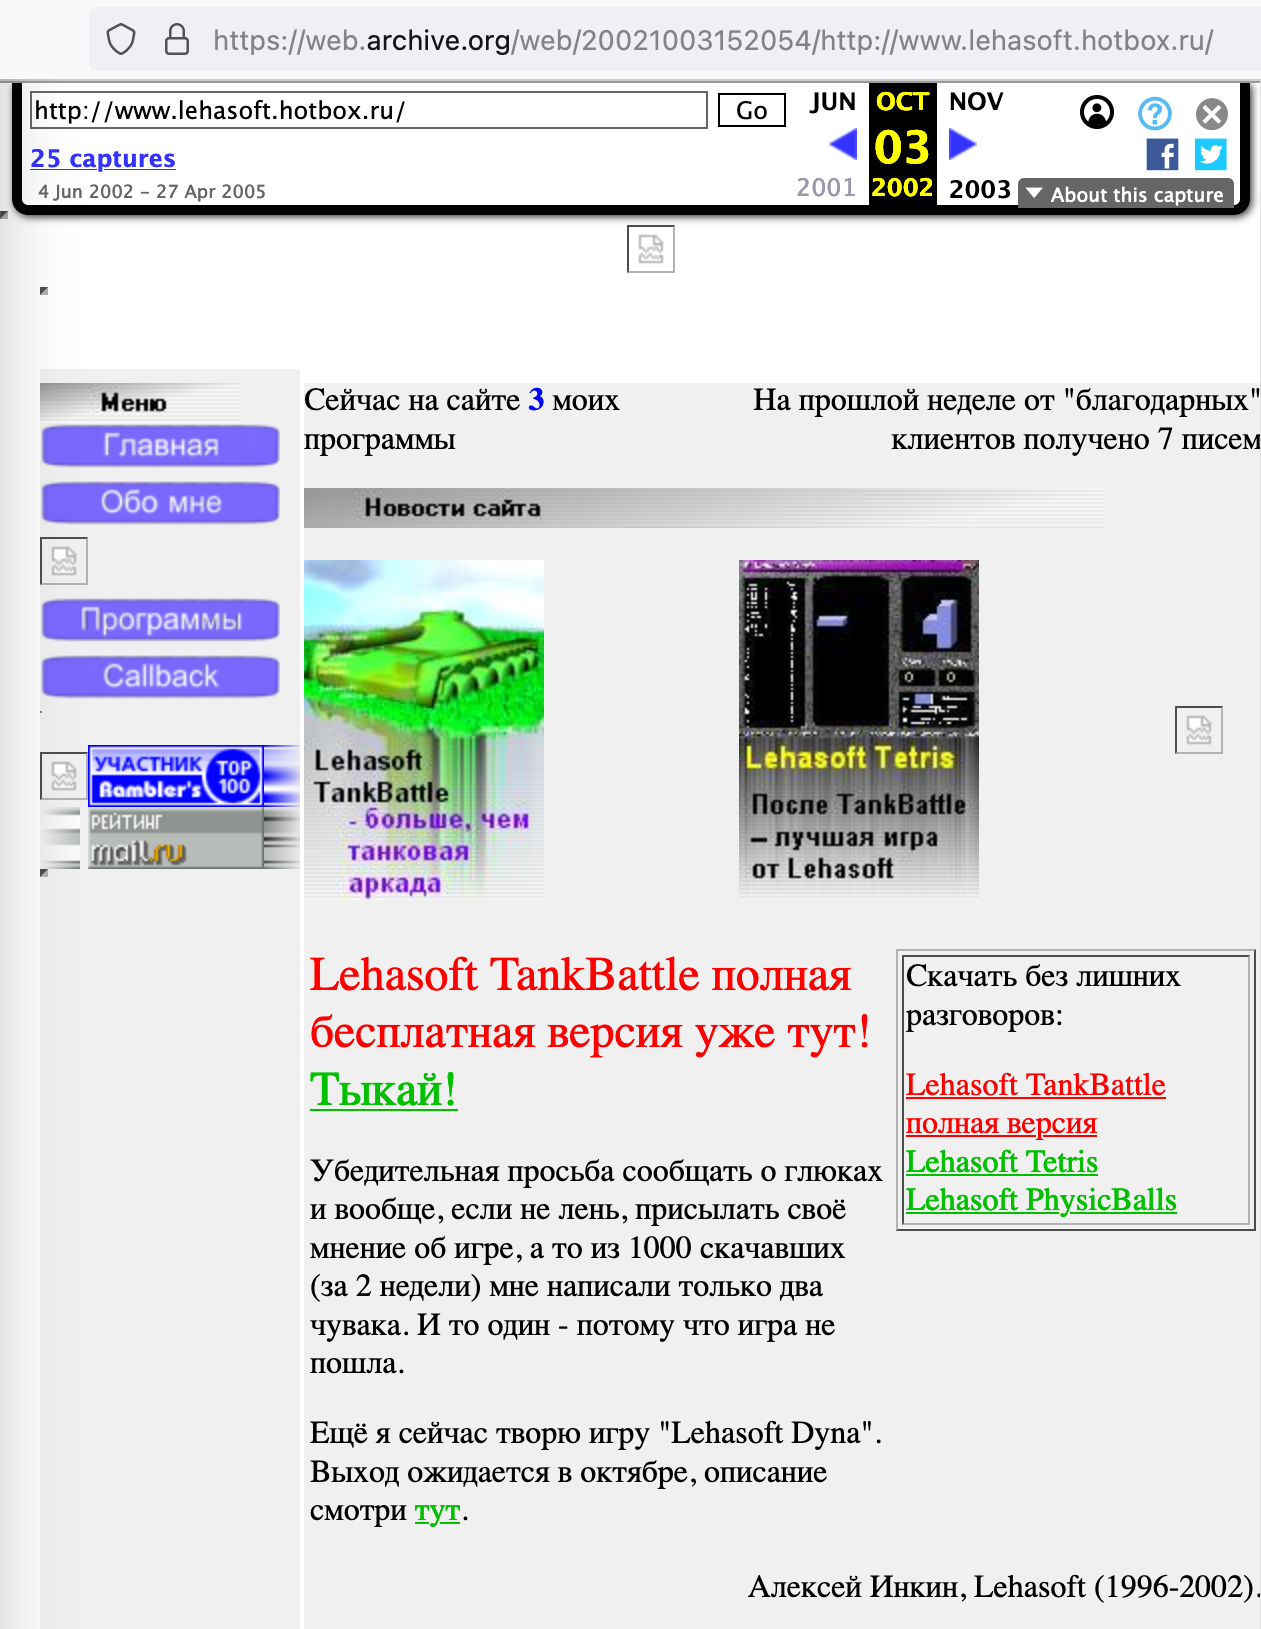
\includegraphics[width=\textwidth]{lehasoft-hotbox}
\end{center}

\pagebreak
